\documentclass{standalone}

\usepackage{package/integrated-circuits-tikz}

\usepackage{siunitx}

\tikzset{
    tip/.style args = {#1 and #2}{
        semithick,
        ->,
        >=stealth,
        shorten >= #1,
        shorten <= #2
    },
    tip/.default = {0pt and 0pt},
}

\definecolor{annotationgray}{RGB}{220,220,220}

\begin{document}
    \begin{tikzpicture}
        [
            node distance = 1.0cm
        ]
        %*************
        % Oscillator *
        %*************
        \node[coordinate] (vcoorigin) at (0, 0) { };
        % resonator
        \node[dot] (cl) at ($(vcoorigin)-(0.8, 0)$) { };
        \node[dot] (cr) at ($(vcoorigin)+(0.8, 0)$) { };
        \draw[wire] (cl) -- ++(-0.5, 0) node[dot] (vleft) { };
        \draw[wire] (cr) -- ++( 0.5, 0) node[dot] (vright) { };
        % main part
        \node[inductor, above = 0.25cm of vcoorigin, anchor = center] (Lres) { };
        \node[capacitor, below = 0.25cm of vcoorigin, anchor = center] (Cres) { };
        \draw[wire] (Lres.west) -| (-0.5, 0) node[dot] (cresl) {} |- (Cres.west);
        \draw[wire] (Lres.east) -| ( 0.5, 0) node[dot] (cresr) {} |- (Cres.east);
        \draw[wire] (cresl) -| (cl);
        \draw[wire] (cresr) -| (cr);
        \begin{scope}[on background layer]
            \fill[rounded corners, fill = annotationgray] ($(Lres.east |- Cres.east)+(0.2, -0.25)$) rectangle ($(Lres.west)+(-0.2, 0.25)$);
            %\draw[rounded corners, thick, densely dotted] ($(Lres.east |- Cres.east)+(0.2, -0.20)$) rectangle ($(Lres.west)+(-0.2, 0.20)$);
        \end{scope}
        % capbank
        \node[eswitch, above = 1cm of vcoorigin, anchor = center] (capswitch) { };
        \node[capacitor, left = 0.25cm of capswitch, anchor = center] (Cbankleft) { };
        \node[capacitor, right = 0.25cm of capswitch, anchor = center] (Cbankright) { };
        \draw[wire] (capswitch.minus) -- (Cbankleft.plus);
        \draw[wire] (capswitch.plus) -- (Cbankright.minus);
        \draw[wire] (Cbankleft.minus) -| (cl);
        \draw[wire] (Cbankright.plus) -| (cr);
        \begin{scope}[on background layer]
            \fill[rounded corners, fill = annotationgray] ($(Cbankleft.west)-(0.2, 0.3)$) rectangle ($(Cbankright.east)+(0.2, 0.3)$);
            \draw[wire] ($(capswitch.center)+(0, 0.3)$) -- coordinate[label = {[font = \scriptsize, xshift = 0pt] right:4}] (cbankbit) ++(0, 0.3) node[port] {};
            \draw[wire] ($(cbankbit)+(-2pt, -2pt)$) -- ($(cbankbit)+(2pt, 2pt)$);
        \end{scope}
        % varactor
        \node[capacitor, circuits/capacitor/variable = true, below = 1cm of vcoorigin, anchor = center] (Cvar) { };
        \draw[wire] (Cvar.minus) -| (cl);
        \draw[wire] (Cvar.plus) -| (cr);
        \begin{scope}[on background layer]
            \fill[rounded corners, fill = annotationgray] ($(Cvar.west)-(0.3, 0.35)$) rectangle ($(Cvar.east)+(0.3, 0.35)$);
        \end{scope}

        % pmos
        \node[pmos, above = 1.74cm of vleft, xscale = -1, anchor = drain] (Pleft) { };
        \node[pmos, above = 1.74cm of vright, anchor = drain] (Pright) { };
        \draw[wire] (Pleft.drain) node[dot] (cpl) { } -- (vleft);
        \draw[wire] (Pright.drain) node[dot] (cpr) { } -- (vright);
        \draw[wire] (cpl) to[angleconnect =  1.0cm and  0.6cm] (Pright.gate);
        \draw[wire] (cpr) to[angleconnect = -1.0cm and -0.6cm] (Pleft.gate);
        \draw[wire] (Pleft.source) -- node[dot] (cum) { } (Pright.source);

        % nmos
        \node[nmos, below = 1.74cm of vleft, anchor = drain, xscale = -1] (Nleft) { };
        \node[nmos, below = 1.74cm of vright, anchor = drain] (Nright) { };
        \draw[wire] (Nleft.drain) node[dot] (cnl) { } -- (vleft);
        \draw[wire] (Nright.drain) node[dot] (cnr) { } -- (vright);
        \draw[wire] (cnl) to[angleconnect =  1.0cm and  0.6cm] (Nright.gate);
        \draw[wire] (cnr) to[angleconnect = -1.0cm and -0.6cm] (Nleft.gate);
        \draw[wire] (Nleft.source) -- node[dot] (clm) { } (Nright.source);

        % current source
        \node[currentsource, above = 0.15cm of cum, label = {[label distance = 0.2cm] left:$I_{\mathrm{osc}}$}] (Ibias) { };
        \draw[wire] (Ibias.east) -- coordinate[label = {[font = \scriptsize, yshift = 2pt] below:4}] (ibiasbit) ++(0.5, 0) node[port] {};
        \draw[wire] ($(ibiasbit)+(-2pt, -2pt)$) -- ($(ibiasbit)+(2pt, 2pt)$);
        \draw[wire] (cum) -- (Ibias.south);

        % power
        \node[ground, below = 0.10cm of clm] (gnd) { };
        \node[vdd, above = 0.25cm of Ibias, label = right:\qty{1.8}{\volt}] (vdd) { };
        \draw[wire] (clm) -- (gnd.north);
        \draw[wire] (Ibias.north) -- (vdd.south);

        %**************
        % Side Images *
        %**************
        % resonator
        \coordinate[right = 3.5cm of vcoorigin] (resonatorinfo);
        \node (resonator) at (resonatorinfo) {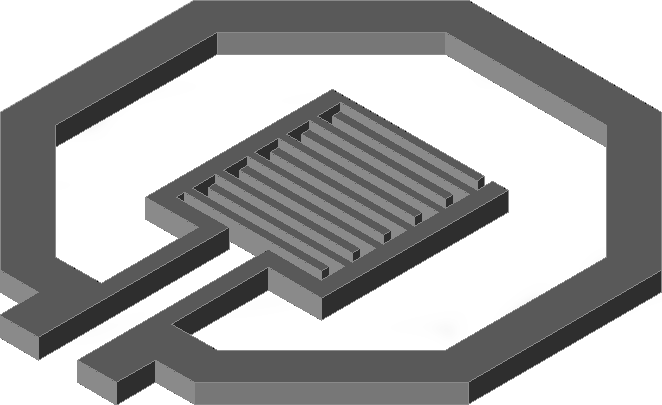
\includegraphics[width=2.5cm]{examples/LC_oscillator_GEMIC_2022_resonator_bw}};
        \begin{scope}[on background layer]
            \draw[rounded corners, fill = annotationgray] ($(resonatorinfo)-(1.8, 0.8)$) rectangle ($(resonatorinfo)+(1.8, 0.8)$);
        \end{scope}
        \draw[tip] ($(Lres.east |- Cres.east)+(0.2, -0.0)$) -- ($(resonatorinfo)+(-1.6, -0.4)$);
        % varactor
        \coordinate[below right = 2.1cm and 3.5cm of vcoorigin] (varactorinfo);
        \node[nmos, left = 0.75cm of varactorinfo, anchor = center] (varactorleft) {};
        \draw[wire] (varactorleft.drain) -| ($(varactorleft.bulk)+(0.2, 0)$) node[dot] (vcl) {} |- (varactorleft.source);
        \node[nmos, right = 0.75cm of varactorinfo, xscale = -1, anchor = center] (varactorright) {};
        \draw[wire] (varactorright.drain) -| ($(varactorright.bulk)+(-0.2, 0)$) node[dot] (vcr) {} |- (varactorright.source);
        \draw[wire] (vcl) -- node[dot] (vcc) {} (vcr);
        \draw[wire] (varactorleft.gate) -- ++(-0.5, 0) node[port, label = above:$v_+$] (vvaracleft) {};
        \draw[wire] (varactorright.gate) -- ++(0.5, 0) node[port, label = above:$v_-$] (vvaracright) {};
        \draw[wire] (vcc) -- ++(0, 0.5) node[port, label=above:$V_{\mathrm{ctrl}}$] (vctrlport) {};
        \coordinate[above = 0.4cm of vctrlport] (varactop);
        \begin{scope}[on background layer]
            \draw[rounded corners, fill = annotationgray] ($(varactorinfo)-(1.8, 0.6)$) rectangle ($(varactorinfo)+(1.8, 1.1)$);
        \end{scope}
        \draw[tip] ($(Cvar.east)+(0.3, -0.2)$) -- ($(varactorinfo)+(-1.6, 0.6)$);
        % capbank
        \coordinate[above right = 1.5cm and 3.5cm of vcoorigin] (capbankinfo);
        \node[nmos, circuits/mosfet/drain length = 0cm, circuits/mosfet/source length=0cm, rotate = -90, above = of capbankinfo, anchor = center] (Nmain) {};
        \node[capacitor, left = 0.8cm of Nmain.source] (cleft) {};
        \node[capacitor, right = 0.8cm of Nmain.drain] (cright) {};
        \draw[wire] (cleft.plus) -- node[dot] (cl) {} (Nmain.source);
        \draw[wire] (cright.minus) -- node[dot] (cr) {} (Nmain.drain);
        \begin{scope}[circuits/mosfet/drain length = 0.3cm]
            \node[nmos, anchor = drain] (Nauxl) at (cl) {};
            \node[nmos, anchor = drain, xmirror] (Nauxr) at (cr) {};
        \end{scope}
        \draw[wire] (Nauxl.source) -- node[dot] (cg) {} (Nauxr.source);
        \node[ground, below = 0.1cm] at (cg) (gnd) {};
        \draw[wire] (cg) -- (gnd.north);
        \node[port, left = 0.1cm of cleft, label = { above:$v_+$}] (pleft) {};
        \node[port, right = 0.1cm of cright, label = {above:$v_-$}] (pright) {};
        \draw[wire] (pleft) -- (cleft.minus);
        \draw[wire] (pright) -- (cright.plus);
        \node[port, above = 0.1cm of Nmain.gate, label = { above:$b_x$}] (penable1) {};
        \node[port, left = 0.1cm of Nauxl.gate, label = { left:$b_x$}] (penable2) {};
        \node[port, right = 0.1cm of Nauxr.gate, label = { right:$b_x$}] (penable3) {};
        \draw[wire] (penable1) -- (Nmain.gate);
        \draw[wire] (penable2) -- (Nauxl.gate);
        \draw[wire] (penable3) -- (Nauxr.gate);
        \begin{scope}[on background layer]
            \draw[rounded corners, fill = annotationgray] ($(capbankinfo)-(1.8, 0.5)$) rectangle ($(capbankinfo)+(1.8, 1.85)$);
            \node[anchor = north west] at ($(capbankinfo)+(-1.8, 1.85)$) { $4\times$ };
        \end{scope}
        \draw[tip] ($(Cbankright.east)+(0.2, 0.2)$) -- ($(capbankinfo)+(-1.6, -0.2)$);
    \end{tikzpicture}
\end{document}
